% RadianceSwap technical report. Build: make -C docs/whitepaper pdf
\documentclass[10pt,conference,a4paper]{IEEEtran}
\IEEEoverridecommandlockouts

\usepackage[T1]{fontenc}
\usepackage[utf8]{inputenc}
\usepackage{amsmath,amssymb}
\usepackage{microtype}
\usepackage{graphicx}
\usepackage{booktabs}
\usepackage{multirow}
\usepackage{array}
\usepackage{xcolor}
\usepackage{cite}
\usepackage{listings}
\usepackage{algorithm}
\usepackage{algpseudocode}
\usepackage{tikz}
\usepackage{pgfplots}
\usepackage[hidelinks]{hyperref}
\pgfplotsset{compat=1.18}
\usetikzlibrary{arrows.meta,positioning,fit,backgrounds,calc}

% ---------------------------------------------------------------- colours and styles
\definecolor{cA}{HTML}{2A78D6}   % series 1
\definecolor{cB}{HTML}{EB6834}   % series 2
\definecolor{cC}{HTML}{1BAF7A}   % series 3
\definecolor{ink}{HTML}{3A3936}
\definecolor{soft}{HTML}{8A8983}
\definecolor{panel}{HTML}{F2F1ED}

\pgfplotsset{
  paper/.style={
    width=0.97\columnwidth, height=4.2cm,
    tick label style={font=\scriptsize}, label style={font=\footnotesize},
    legend style={font=\scriptsize, draw=none, fill=none},
    axis line style={ink!70}, tick style={ink!70},
    major grid style={ink!12}, ymajorgrids=false, xmajorgrids=true,
    every node near coord/.append style={font=\scriptsize, text=ink},
  },
}
\tikzset{
  box/.style={draw=ink!70, fill=white, rounded corners=2pt, align=center, font=\footnotesize, inner sep=3pt},
  boxA/.style={box, draw=cA, fill=cA!8},
  boxB/.style={box, draw=cB, fill=cB!8},
  boxC/.style={box, draw=cC, fill=cC!8},
  boxG/.style={box, fill=panel},
  arr/.style={-{Stealth[length=1.8mm]}, semithick, draw=ink},
  darr/.style={arr, dashed},
  lab/.style={font=\scriptsize, text=ink, fill=white, inner sep=1pt},
}

\lstset{basicstyle=\ttfamily\scriptsize, columns=fullflexible, keepspaces=true, breaklines=true,
  frame=lines, rulecolor=\color{ink!40}, showstringspaces=false, upquote=true, aboveskip=4pt, belowskip=4pt}

\newcommand{\code}[1]{\texttt{#1}}
\newcommand{\GiB}{\,GiB}
\newcommand{\MiB}{\,MiB}

\begin{document}

\title{RadianceSwap: In-Process Multi-Model\\ LLM Serving with Dynamic VRAM Sharing}

\author{\IEEEauthorblockN{The RadianceSwap Contributors}
\IEEEauthorblockA{\url{https://github.com/Code000-211/RadianceSwap}\\
Technical report, November 2026 (code at \code{86d4503})}}

\maketitle

% ================================================================ abstract
\begin{abstract}
Serving several large language models from one GPU group usually means running one inference
process per model and restarting processes as demand shifts. Each restart re-parses the
checkpoint, re-lays out the weights and rebuilds tokenizer and execution state, and a request for
one model can wait for another model's longest generation. We present RadianceSwap, an extension of
the Radiance inference engine that serves several models from a single process behind one
OpenAI-compatible endpoint. Models are activated by their first request, deactivated when idle, and
kept in host RAM in GPU-ready form, so that re-activation needs no parsing, relayout or disk read.
Several models can be active at once: each runs as an independent runtime, a ticket-based
sequencer gives all tensor-parallel collectives one group-wide order, and a group planner moves
expert, KV-cache and static-weight memory between models at run time. On two AMD Radeon AI PRO
R9700 GPUs (TP\,=\,2), RadianceSwap adds no measurable overhead for a single model
($-0.3\,\%$ to $+0.1\,\%$), re-activates a dense 0.8B model in 2.1\,s, keeps outputs bit-identical
to single-model serving, and lets an idle MoE model hand $\sim$3\GiB\ per card to a busy one within
30\,s. The approach is experimental and was evaluated on one system.
\end{abstract}

\begin{IEEEkeywords}
LLM serving, multi-model inference, GPU memory management, mixture of experts, tensor parallelism
\end{IEEEkeywords}

% ================================================================ 1 intro
\section{Introduction}

Operators of on-premise inference servers increasingly want to offer several models at once: a
large mixture-of-experts (MoE) model for quality, a small dense model for latency, an embedding or
image model beside them. GPU memory, however, rarely holds all of them. The common practice is to
run one inference server per model behind a proxy that starts and stops server processes on demand,
as in llama-swap~\cite{llamaswap}. Two costs follow from that design. First, every switch pays the
full start-up path: checkpoint parsing, weight relayout and the construction of tokenizer, chat
template and execution plans; for a 113.6\GiB\ MoE container this exceeds a minute. Second, when
only one model fits at a time, a request for model B waits for model A's longest running
generation, which is unbounded, unless running generations are aborted.

RadianceSwap removes both costs inside the Radiance engine~\cite{radiance}. A single process owns
the HTTP listener and the GPU group; models come and go as \emph{runtimes} within it. The design
rests on three decisions, recorded as architecture decision records (ADRs) in the repository:
switching happens in process (ADR~0001); several models may be active at the same time and share
VRAM (ADR~0002); and active models run as separate, truly parallel runtimes whose collectives
follow one group-wide order (ADR~0003).

This report makes the following contributions:
\begin{itemize}
  \item A \textbf{model lifecycle} with a host-resident, GPU-ready \emph{prepared store} that turns
        re-activation into an upload without parsing, relayout or disk I/O, together with a
        host-memory budget that refuses an activation before allocation instead of triggering the
        kernel's OOM killer (\S\ref{sec:lifecycle}, \S\ref{sec:host}).
  \item \textbf{Run-time VRAM sharing} between active models: a heat-driven group planner for
        expert memory, an elastic expert slab that returns memory physically, cross-model KV-cache
        lending, and streaming of static weights from host RAM when a model does not fit
        (\S\ref{sec:vram}).
  \item A \textbf{collective sequencer} that prevents cross-model deadlock of spinning all-reduce
        kernels on a tensor-parallel group (\S\ref{sec:collectives}).
  \item An \textbf{evaluation} on two AMD GPUs covering overhead, activation latency, time to first
        token, concurrency, memory movement, and four defects found during acceptance
        (\S\ref{sec:eval}), and a comparison with process-swapping proxies (\S\ref{sec:related}).
\end{itemize}

Without the \code{-{}-manifest} option, Radiance behaves exactly as before; everything described
here applies only to manifest mode.

% ================================================================ 2 background
\section{Background}

\paragraph{Radiance} Radiance is a C++ inference engine with architecture and kernel plugins and a
ROCm/HIP device layer~\cite{radiance}. It loads \code{.rad} containers or Hugging Face checkpoints,
converts them into the kernels' packed layouts, and serves an OpenAI-compatible API. Its placement
layer already supports tiered expert residency: a planner fills a fixed number of VRAM expert slots,
and a mover promotes and demotes experts by observed routing \emph{heat}, serving the rest from a
pinned host pool.

\paragraph{Tensor parallelism} With tensor parallelism (TP)~\cite{megatron}, each layer's weights
are sharded across the ranks of a GPU group, and partial results are combined by an all-reduce after
attention and MLP blocks. Radiance's all-reduce kernels busy-wait on a flag written by the peer
rank. Two independent models issuing such collectives concurrently can therefore deadlock if the
ranks disagree on the order.

\paragraph{Mixture of experts} MoE layers~\cite{shazeer2017,fedus2022} route each token to a small
subset of experts. Expert popularity is skewed and changes with the workload, which makes experts
the natural unit for moving memory between models: a cold expert can be served from host memory at
low cost, as exploited by offloading systems~\cite{eliseev2023,flexgen,dsinference}.

% ================================================================ 3 design
\section{Design}\label{sec:design}

\begin{figure*}[t]
\centering
\resizebox{\textwidth}{!}{%
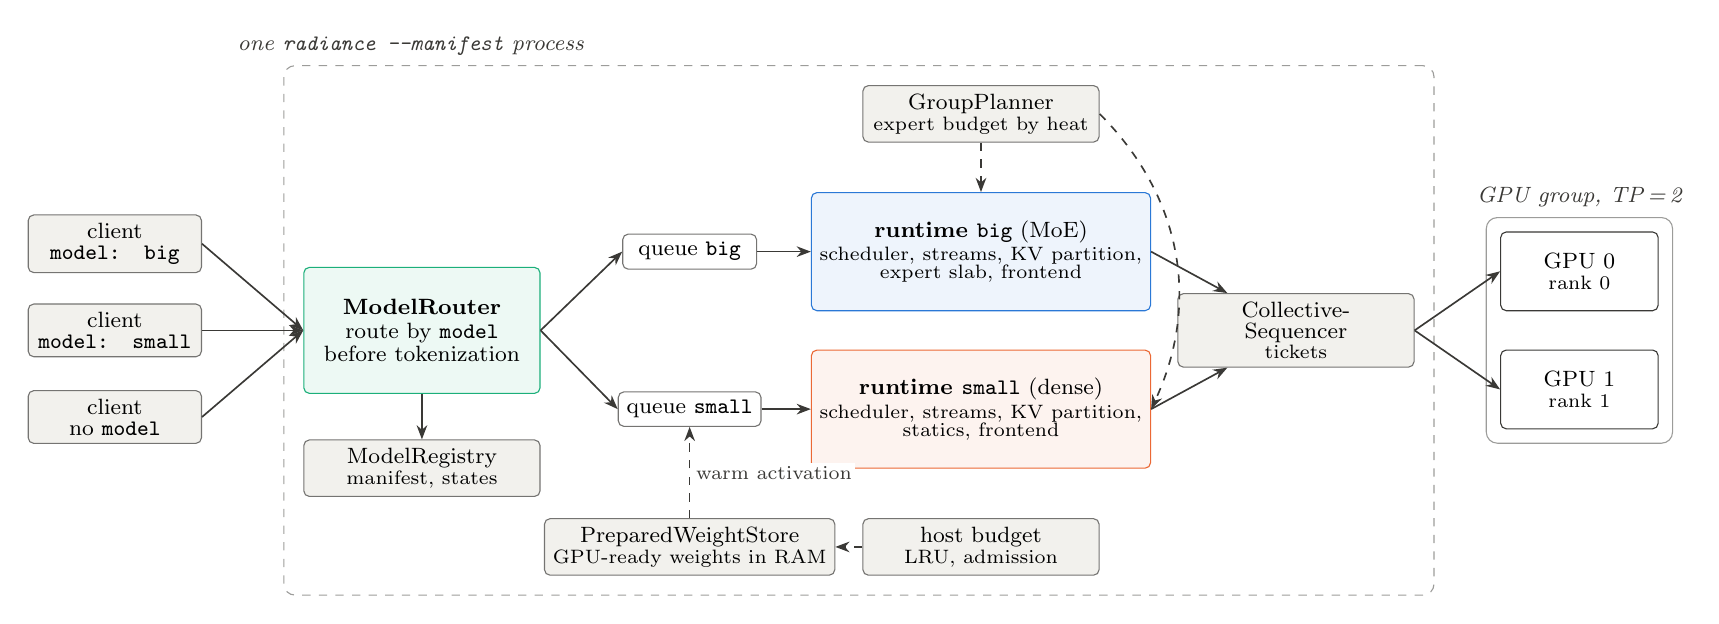
\begin{tikzpicture}[node distance=6mm]
  % clients
  \node[boxG, minimum width=22mm] (c1) at (0, 1.1) {client\\[-2pt]\code{model: big}};
  \node[boxG, minimum width=22mm] (c2) at (0, 0)   {client\\[-2pt]\code{model: small}};
  \node[boxG, minimum width=22mm] (c3) at (0,-1.1) {client\\[-2pt]no \code{model}};
  % router
  \node[boxC, minimum width=30mm, minimum height=16mm] (router) at (3.9,0)
     {\textbf{ModelRouter}\\[-1pt]route by \code{model}\\[-1pt]before tokenization};
  \node[boxG, minimum width=30mm] (reg) at (3.9,-1.75) {ModelRegistry\\[-2pt]\scriptsize manifest, states};
  % queues
  \node[box, minimum width=17mm] (qa) at (7.3, 1.0) {queue \code{big}};
  \node[box, minimum width=17mm] (qb) at (7.3,-1.0) {queue \code{small}};
  % runtimes
  \node[boxA, minimum width=36mm, minimum height=15mm] (ra) at (11.0, 1.0)
     {\textbf{runtime \code{big}} (MoE)\\[-1pt]\scriptsize scheduler, streams, KV partition,\\[-3pt]\scriptsize expert slab, frontend};
  \node[boxB, minimum width=36mm, minimum height=15mm] (rb) at (11.0,-1.0)
     {\textbf{runtime \code{small}} (dense)\\[-1pt]\scriptsize scheduler, streams, KV partition,\\[-3pt]\scriptsize statics, frontend};
  % services
  \node[boxG, minimum width=30mm] (gp) at (11.0, 2.75) {GroupPlanner\\[-2pt]\scriptsize expert budget by heat};
  \node[boxG, minimum width=30mm] (cs) at (15.0, 0) {Collective-\\[-2pt]Sequencer\\[-2pt]\scriptsize tickets};
  \node[boxG, minimum width=30mm] (st) at (7.3,-2.75) {PreparedWeightStore\\[-2pt]\scriptsize GPU-ready weights in RAM};
  \node[boxG, minimum width=30mm] (hb) at (11.0,-2.75) {host budget\\[-2pt]\scriptsize LRU, admission};
  % gpu group
  \node[box, draw=ink, minimum width=20mm, minimum height=10mm] (g0) at (18.6, 0.75) {GPU 0\\[-2pt]\scriptsize rank 0};
  \node[box, draw=ink, minimum width=20mm, minimum height=10mm] (g1) at (18.6,-0.75) {GPU 1\\[-2pt]\scriptsize rank 1};
  \begin{scope}[on background layer]
    \node[draw=ink!50, dashed, rounded corners=4pt, fit=(router)(reg)(gp)(cs)(st)(hb)(ra)(rb), inner sep=7pt,
          label={[font=\footnotesize\itshape, text=ink]above left:one \code{radiance -{}-manifest} process}] (proc) {};
    \node[draw=ink!50, rounded corners=4pt, fit=(g0)(g1), inner sep=5pt,
          label={[font=\footnotesize\itshape, text=ink]above:GPU group, TP\,=\,2}] (grp) {};
  \end{scope}
  % edges
  \foreach \c in {c1,c2,c3} \draw[arr] (\c.east) -- (router.west);
  \draw[arr] (router) -- (reg);
  \draw[arr] (router.east) -- (qa.west);
  \draw[arr] (router.east) -- (qb.west);
  \draw[arr] (qa) -- (ra);
  \draw[arr] (qb) -- (rb);
  \draw[darr] (st.north) -- node[lab, right=1pt]{warm activation} (qb.south);
  \draw[darr] (gp) -- (ra);
  \draw[darr] (gp.east) to[bend left=35] (rb.east);
  \draw[arr] (ra.east) -- (cs);
  \draw[arr] (rb.east) -- (cs);
  \draw[arr] (cs.east) -- (g0.west);
  \draw[arr] (cs.east) -- (g1.west);
  \draw[darr] (hb) -- (st);
\end{tikzpicture}}
\caption{Architecture of RadianceSwap. One process owns the listener and the GPU group. The router
resolves the model before any tokenizer is touched; each active model is an independent runtime.
Shared services decide expert budgets (GroupPlanner), order collectives (CollectiveSequencer) and
hold deactivated models in GPU-ready form (PreparedWeightStore) under a host-memory budget.}
\label{fig:arch}
\end{figure*}

Fig.~\ref{fig:arch} shows the components. A JSON \emph{manifest} names the GPU group, cache
policies and the models with their per-model engine options; it replaces \code{-{}-model}. Unknown
keys are rejected, so a typo cannot become a silent default.

\subsection{Process model and routing}

HTTP listener, plugin and tool registries and the coordination of the GPU group belong to the
process; a model runtime cannot close them (ADR~0001). The \emph{ModelRouter} reads a request's
\code{model} field \emph{before} tokenization, so every request uses the tokenizer, chat template,
grammar and context limit of its own model. A request without \code{model} goes to the default
model; an unknown id yields HTTP~404. Requests for a model that is not active join that model's
bounded queue (64 by default, HTTP~429 beyond). All concurrent first requests share a single
activation, which runs on its own thread so that no HTTP thread builds an engine. Image and audio
requests are routed the same way; video jobs and WebSocket sessions are refused with HTTP~501 in
manifest mode, and LoRA adapters are rejected at start-up because an adapter belongs to one base
model.

\subsection{Model lifecycle}\label{sec:lifecycle}

\begin{figure}[t]
\centering
\resizebox{\columnwidth}{!}{%
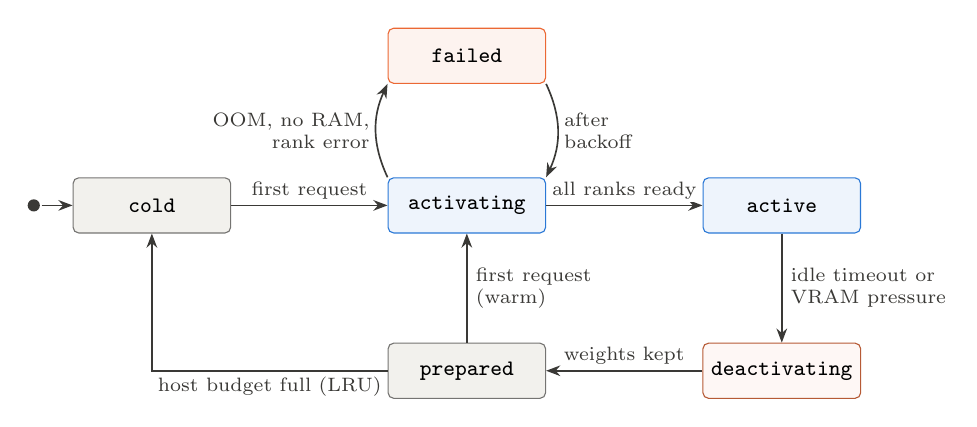
\begin{tikzpicture}[st/.style={box, minimum width=20mm, minimum height=7mm}]
  \node[st, fill=panel] (cold) at (0,0) {\code{cold}};
  \node[st, draw=cA, fill=cA!8] (act) at (4,0) {\code{activating}};
  \node[st, draw=cA, fill=cA!8] (active) at (8,0) {\code{active}};
  \node[st, draw=cB, fill=cB!8] (fail) at (4,1.9) {\code{failed}};
  \node[st, draw=cB!70!ink, fill=cB!5] (deact) at (8,-2.1) {\code{deactivating}};
  \node[st, fill=panel] (prep) at (4,-2.1) {\code{prepared}};
  \fill[ink] (-1.5,0) circle (2.2pt); \draw[arr] (-1.4,0) -- (cold);
  \draw[arr] (cold) -- node[lab, above=1pt]{first request} (act);
  \draw[arr] (act) -- node[lab, above=1pt]{all ranks ready} (active);
  \draw[arr] (act.north west) to[bend left=25] node[lab, left=1pt, align=right]{OOM, no RAM,\\rank error} (fail.south west);
  \draw[arr] (fail.south east) to[bend left=25] node[lab, right=1pt, align=left]{after\\backoff} (act.north east);
  \draw[arr] (active) -- node[lab, right=2pt, align=left]{idle timeout or\\VRAM pressure} (deact);
  \draw[arr] (deact) -- node[lab, above=1pt]{weights kept} (prep);
  \draw[arr] (prep) -- node[lab, right=2pt, align=left]{first request\\(warm)} (act);
  \draw[arr] (prep.west) -| node[lab, pos=0.25, below=1pt]{host budget full (LRU)} (cold.south);
\end{tikzpicture}}
\caption{Lifecycle of one model, as reported by \code{/radiance/models}.}
\label{fig:lifecycle}
\end{figure}

Each model moves through the states of Fig.~\ref{fig:lifecycle}. Only the default model is started
with the process; every other model starts \code{cold}. A model is \code{active} only once all ranks
are ready. Deactivation is triggered by an idle timeout or by VRAM pressure. A model is idle only if
no request lies between routing and the end of its response, so a streaming response keeps it busy
until its last chunk; \emph{a running generation is never interrupted}. Deactivation discards KV,
prefix-cache and recurrent state but keeps weights, tokenizer, configuration and expert heat.

Under VRAM pressure, a model that finds the cards full causes the router to deactivate the active
model that has been idle the longest; a model that is generating is never chosen, and one request
triggers at most one such round per configured model. A failed activation (insufficient VRAM or
host memory, a bad container, a rank error) releases every partial allocation on every rank and
leaves other models untouched; retries back off exponentially from 1\,s to 60\,s. A device error
instead marks the whole GPU group unhealthy, since retrying cannot help.

\paragraph{Prepared weight store} The first activation of a model copies its weights, in the packed
form the kernels read, into a process-owned \emph{PreparedWeightStore}. Weights are never
dequantized or requantized. The store holds anonymous process memory rather than references to the
container's page-cache mapping, because the kernel may reclaim page cache at any time; only the
store makes ``the second activation reads no checkpoint bytes'' true. A re-activation from the store
is an upload through a pinned staging ring.

\subsection{Memory hierarchy}

\begin{figure}[t]
\centering
\resizebox{\columnwidth}{!}{%
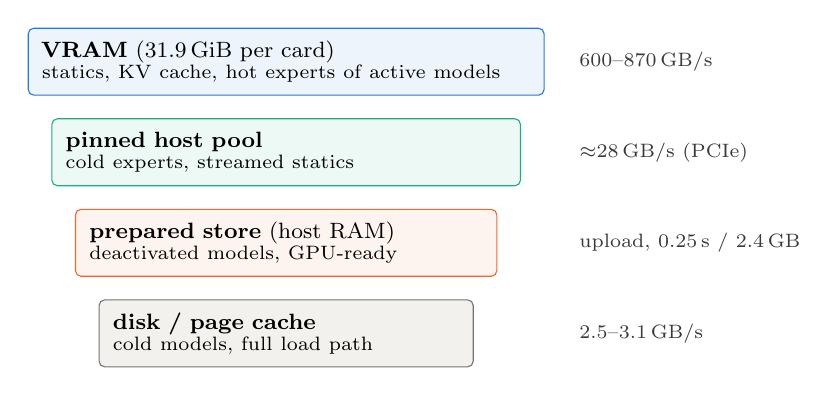
\begin{tikzpicture}[tier/.style={box, minimum height=8.5mm, text width=#1, align=left, inner xsep=5pt}]
  \node[tier=62mm, draw=cA, fill=cA!8] (v) at (0,0) {\textbf{VRAM} (31.9\GiB\ per card)\\[-2pt]\scriptsize statics, KV cache, hot experts of active models};
  \node[tier=56mm, draw=cC, fill=cC!8] (p) at (0,-1.15) {\textbf{pinned host pool}\\[-2pt]\scriptsize cold experts, streamed statics};
  \node[tier=50mm, draw=cB, fill=cB!8] (s) at (0,-2.3) {\textbf{prepared store} (host RAM)\\[-2pt]\scriptsize deactivated models, GPU-ready};
  \node[tier=44mm, fill=panel] (d) at (0,-3.45) {\textbf{disk / page cache}\\[-2pt]\scriptsize cold models, full load path};
  \node[font=\scriptsize, text=ink, anchor=west] at (3.6,0) {600--870\,GB/s};
  \node[font=\scriptsize, text=ink, anchor=west] at (3.6,-1.15) {$\approx$28\,GB/s (PCIe)};
  \node[font=\scriptsize, text=ink, anchor=west] at (3.6,-2.3) {upload, 0.25\,s / 2.4\,GB};
  \node[font=\scriptsize, text=ink, anchor=west] at (3.6,-3.45) {2.5--3.1\,GB/s};
\end{tikzpicture}}
\caption{Where a model's weights can live, with bandwidths measured on the test system.}
\label{fig:tiers}
\end{figure}

Fig.~\ref{fig:tiers} summarizes the tiers. The ratio between VRAM and PCIe bandwidth, roughly
20--30$\times$, governs every trade-off below: anything read over PCIe during decoding is expensive,
so host-resident weights are a bridge, not a steady state.

\subsection{Sharing VRAM between active models}\label{sec:vram}

Each model is assigned a fixed \emph{share} of the free VRAM of the group's tightest card, less
headroom, divided by $\min(n, m)$ where $n$ is the number of models and $m$ is
\code{max\_active\_models}. The share caps the model's static weights, KV cache and experts. Inside
the shares, four mechanisms move memory at run time (Fig.~\ref{fig:vram}).

\begin{figure}[t]
\centering
\resizebox{\columnwidth}{!}{%
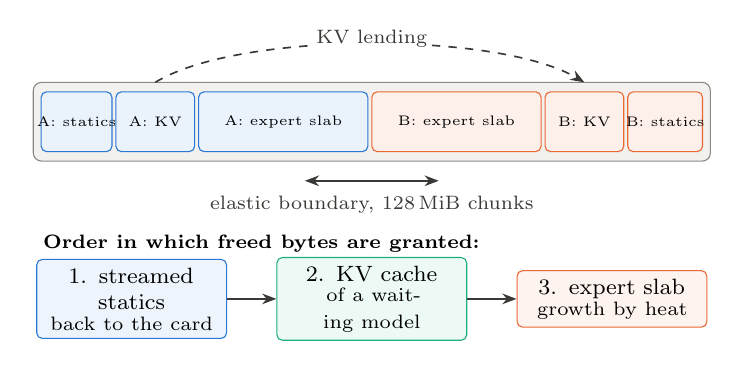
\begin{tikzpicture}
  \draw[ink!60, rounded corners=3pt, fill=panel] (0,0) rectangle (8.6,1.0);
  \foreach \x/\w/\c/\t in {0.1/0.9/cA/A: statics, 1.05/1.0/cA/A: KV, 2.1/2.15/cA/A: expert slab,
                          4.3/2.15/cB/B: expert slab, 6.5/1.0/cB/B: KV, 7.55/0.95/cB/B: statics}{
     \draw[draw=\c, fill=\c!10, rounded corners=2pt] (\x,0.12) rectangle ++(\w,0.76);
     \node[font=\tiny] at (\x+\w/2,0.5) {\t};
  }
  \draw[{Stealth[length=1.8mm]}-{Stealth[length=1.8mm]}, semithick, draw=ink] (3.45,-0.25) -- (5.15,-0.25);
  \node[font=\scriptsize, text=ink] at (4.3,-0.55) {elastic boundary, 128\MiB\ chunks};
  \draw[darr] (1.55,1.0) .. controls (2.6,1.65) and (5.9,1.65) .. (7.0,1.0);
  \node[lab] at (4.3,1.55) {KV lending};
  \node[font=\scriptsize\bfseries, anchor=west] at (0,-1.05) {Order in which freed bytes are granted:};
  \node[boxA, text width=22mm] (o1) at (1.25,-1.75) {1. streamed statics\\[-2pt]\scriptsize back to the card};
  \node[boxC, text width=22mm] (o2) at (4.3,-1.75) {2. KV cache\\[-2pt]\scriptsize of a waiting model};
  \node[boxB, text width=22mm] (o3) at (7.35,-1.75) {3. expert slab\\[-2pt]\scriptsize growth by heat};
  \draw[arr] (o1) -- (o2); \draw[arr] (o2) -- (o3);
\end{tikzpicture}}
\caption{Two active models on one card (schematic). Freed bytes go first to streamed static
weights, then to the KV cache of a model with waiting prompts, and last to expert-slab growth.}
\label{fig:vram}
\end{figure}

\paragraph{Group planner} The expert bytes a model's share leaves are its \emph{offer}; the group's
expert pool $P$ is the sum of the offers. Algorithm~\ref{alg:planner} computes per-rank targets.
Every model keeps a minimum, the larger of its \emph{expert floor} (what its host pool cannot hold)
and a fraction of the equal share $P/n$. The remainder goes to the most valuable expert units of the
whole group, where an expert's worth is its heat times its bytes per byte of slot it occupies,
which makes models with different expert sizes comparable. Running models apply new targets only
at step boundaries, by capping their mover's resident slots. A model alone in the group receives
exactly its offer, so single-model behaviour is unchanged.

\begin{algorithm}[t]
\caption{Expert budget per rank (GroupPlanner)}\label{alg:planner}
\small
\begin{algorithmic}[1]
\Require models $i=1..n$ with offer $o_i$, floor $f_i$, expert plane $E_i$, heat per unit
\State $P \gets \sum_i o_i$; \quad $s \gets \textit{min\_share}\cdot P/n$
\For{each model $i$}
  \State $k_i \gets \min(\max(f_i, s),\ |E_i|)$ \Comment{guaranteed minimum}
\EndFor
\State $R \gets P - \sum_i k_i$
\State $U \gets$ expert units of all models, by $w(u)=\frac{\mathit{heat}(u)\cdot \mathit{bytes}(u)}{\mathit{slot}(u)}$, desc.
\For{$u \in U$ \textbf{while} $R>0$}
  \State $i \gets \mathrm{owner}(u)$
  \If{$k_i + \mathit{slot}(u) \le c_i$} \Comment{$c_i=o_i$, or $P$ if elastic}
     \State $k_i \gets k_i + \mathit{slot}(u)$; \quad $R \gets R - \mathit{slot}(u)$
  \EndIf
\EndFor
\State \Return targets $k_i$ \Comment{ties share room by bytes}
\end{algorithmic}
\end{algorithm}

\paragraph{Elastic expert slab} Logical targets alone do not move memory: a shrinking model's slab
would remain one reservation. On cards with virtual-memory management and in manifests with more
than one model, the expert slab is therefore \emph{elastic}. It is mapped in chunks of about
128\MiB; a model may be granted up to the whole pool, but growth is paid only from chunks no member
holds, and the receiver is granted bytes only after the giver reports their release, so the sum of
committed slabs never exceeds the pool. Heat of an idle model halves every 4\,s and counts as cold
after 20\,s, so an idle model shrinks to its minimum. Every chunk is mapped on \emph{fresh} virtual
address space; \S\ref{sec:lessons} explains why. Each rank reserves 8\,TiB of address space per
model, about 65{,}000 chunk changes, after which the slab degrades to logical shrinking.

\paragraph{Cross-model KV lending} A model's share fixes only its initial KV cache (its
\emph{carve}); its ceiling is the context length times the number of sequences. When running or
waiting prompts need more blocks than the carve holds, the cache claims chunks of 128--256\MiB\
(32{,}768 tokens per growing group) from the group's expert pool. The planner takes the bytes from
the coldest experts of any model, each model keeping its minimum, and grants them once the pages are
back. Running sequences are never touched, and a chunk is returned five seconds after demand ends.

\paragraph{Static-weight streaming} If a model's non-expert weights do not fit the VRAM left to it,
it starts anyway: what does not fit stays in the pinned host pool and is read over PCIe, zero-copy
for decode and through a staged ring for prefill. Output is bit-identical. As soon as VRAM frees up,
the streamed weights move to the card, and they are first in line for freed bytes
(Fig.~\ref{fig:vram}). Deterministic mode refuses streamed statics, because prefill without a stager
would read weights in place over PCIe.

\paragraph{Heat warm-up} A deactivated model keeps its expert heat for the lifetime of the
process. With a warm-up budget, the next activation ranks experts by that heat and places the
hottest on the card at load time, instead of starting from the container's static profile.

\subsection{Parallel runtimes and collective ordering}\label{sec:collectives}

Each active model owns its streams, threads, contexts, pools and collective buffers per rank, and
its forward passes run truly in parallel with other models' (ADR~0003). The danger lies in the
all-reduce kernels, which spin on a peer flag: if rank~0 enters model A's all-reduce while rank~1
enters model B's, both spin forever. RadianceSwap applies the classical remedy of imposing a total
order on resource acquisition~\cite{havender1968}: a process-wide \emph{CollectiveSequencer}
assigns monotonic tickets on rank~0, and all other ranks issue their collectives in that exact
sequence (Fig.~\ref{fig:collective}). A device-side event chain enforces the order on the streams
without stalling the host, and with a single registered engine the sequencer reduces to a relaxed
atomic check.

\begin{figure}[t]
\centering
\resizebox{\columnwidth}{!}{%
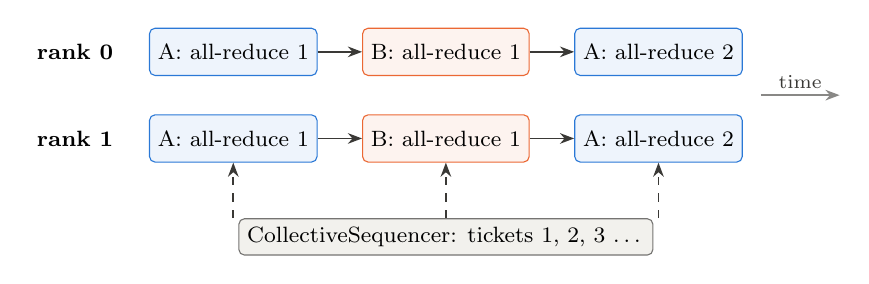
\begin{tikzpicture}[a/.style={boxA, minimum width=21mm, minimum height=6mm}, b/.style={boxB, minimum width=21mm, minimum height=6mm}]
  \foreach \y/\r/\k in {0/rank 0/r0, -1.1/rank 1/r1} {
    \node[font=\footnotesize\bfseries, anchor=east] at (-0.2,\y) {\r};
    \node[a] (x1\k) at (1.2,\y) {A: all-reduce 1};
    \node[b] (x2\k) at (3.9,\y) {B: all-reduce 1};
    \node[a] (x3\k) at (6.6,\y) {A: all-reduce 2};
    \draw[arr] (x1\k) -- (x2\k); \draw[arr] (x2\k) -- (x3\k);
  }
  \node[boxG, minimum width=40mm] (seq) at (3.9,-2.35) {CollectiveSequencer: tickets 1, 2, 3 \dots};
  \draw[darr] (seq.north -| x1r1) -- (x1r1.south);
  \draw[darr] (seq.north -| x2r1) -- (x2r1.south);
  \draw[darr] (seq.north -| x3r1) -- (x3r1.south);
  \draw[arr, draw=ink!60] (7.9,-0.55) -- node[lab, above=1pt]{time} (8.9,-0.55);
\end{tikzpicture}}
\caption{All collectives of all models follow one ticket order, identical on every rank, so no rank
can spin on model A while its peer has entered model B.}
\label{fig:collective}
\end{figure}

The cost is that two models never communicate at the same time. Two busy models therefore share,
rather than add, the communication capacity of the group; the benefit is that the second model is
served without waiting for the first.

\subsection{Host-memory budget and admission control}\label{sec:host}

Host RAM is the binding constraint for large MoE models, because an active model's weights exist
twice: on the card (or in its host pool) and in the prepared store. RadianceSwap books three kinds of
host memory against \code{cache.host\_budget\_mib}: store copies, the host pools of active models
(enlarged by streaming), and load staging. Page cache is never counted. When a booking does not fit,
the longest-idle prepared model is dropped to \code{cold} (LRU~\cite{denning1968}), then the store
copy of an active model, and finally the activating model's own copy. After planning and
\emph{before} allocating, an activation checks its whole host bill against the budget,
\code{MemAvailable}, all enclosing memory cgroups and a headroom; if it still does not fit, the
activation is refused with HTTP~503 and nothing that runs is affected. Before this check, a streaming
model beside a 138\GiB\ MoE ended in a kernel kill of the whole process. A practical sizing rule is
\begin{equation*}
\begin{aligned}
\mathrm{RAM} \gtrsim{} & \textstyle\sum \text{store copies} + \sum \text{active host pools}\\
 & + \text{staging} + \text{headroom}.
\end{aligned}
\end{equation*}

% ================================================================ 4 implementation
\section{Implementation}

RadianceSwap is implemented in C++20 and HIP within the Radiance tree. The main components are the
\code{ModelRegistry} (manifest parsing and per-model records), the \code{ModelRouter} (routing,
queues, activation threads, idle and pressure deactivation), the \code{PreparedWeightStore}
(\code{core/model/weight\_store.h}), the \code{GroupPlanner} (\code{core/place/group\_planner.cpp}),
which hands each engine a byte budget that its existing planner and mover fill, so that there is no
second placement algorithm, and the \code{CollectiveSequencer}
(\code{core/runtime/collective\_sequencer.cpp}). Enabling the lifecycle required splitting the
engine's \code{serve()} into execution start/stop and independent HTTP serving, and turning
stack-local bridges into a lifetime-managed per-model frontend whose leases keep tokenizer and
response sinks valid across a deactivation.

Testing follows three seams. HTTP behaviour is tested through \code{Router::dispatch} with fake model
runtimes (routing, single activation under concurrency, cancellation while waiting, idle timeout, LRU,
rollback, metrics, LoRA rejection). The group planner is tested directly (heat allocation, minima,
slot release, KV reclaim, streaming fallback). GPU acceptance runs on real hardware
(\S\ref{sec:eval}).

% ================================================================ 5 evaluation
\section{Evaluation}\label{sec:eval}

\paragraph{Setup} All measurements were taken on 2$\times$ AMD Radeon AI PRO R9700 (gfx1201,
31.86\GiB\ each) with TP\,=\,2, a host with 48 vCPUs and 170\GiB\ RAM, and a build for gfx1201. The
dense model is Qwen3.5-0.8B (2.4\,GB of weights); the MoE model is Qwen3.8-Flash-Next, a
113.6\GiB\ container with 67.5\GiB\ of weights and a 47.7\GiB\ memory-mapped n-gram table.
C1 denotes one request generating 256 tokens with \code{ignore\_eos}; C8 denotes eight concurrent
requests, aggregated. Unless stated otherwise each value is the min--max range over three
repetitions. All numbers are taken from the repository's acceptance record
(\code{docs/swap/gpu-acceptance.md}); none were re-measured for this report.

\subsection{Overhead}

\begin{table}[t]
\caption{Single-model overhead: unmodified engine (main) vs.\ RadianceSwap, \code{-{}-model} mode, TP\,=\,2. Throughput in tok/s.}
\label{tab:overhead}
\centering\footnotesize
\setlength{\tabcolsep}{4pt}
\begin{tabular}{@{}llrrr@{}}
\toprule
Model & Build & C1 & C8 & Prefill \\
\midrule
\multirow{2}{*}{Dense 0.8B} & main & 325--332 & 2032--2056 & 57{,}000--65{,}100 \\
                            & RadianceSwap & 326--333 & 2015--2039 & 57{,}300--64{,}700 \\
\midrule
\multirow{2}{*}{MoE, determ.} & main & 73.8--77.7 & 129--151 & 4645--4866 \\
                              & RadianceSwap & 72.8--89.0 & 137--226 & 4697--5150 \\
\bottomrule
\end{tabular}
\end{table}

Table~\ref{tab:overhead} compares single-model serving before and after the changes. Dense C1 and
C8 agree within 1\,\%; prefill varies by $\pm$5\,\% from run to run in both builds. A manifest that
holds one model matches \code{-{}-model} within $-0.3\,\%$ to $+0.1\,\%$. Outputs are identical to
\code{-{}-model} for greedy decoding, seeded sampling ($T=0.8$, top-$p=0.9$), streaming, a 2{,}421-token
prompt and MTP speculation, for dense and MoE models, also while another model is active.

\subsection{Activation latency}

\begin{figure}[t]
\centering
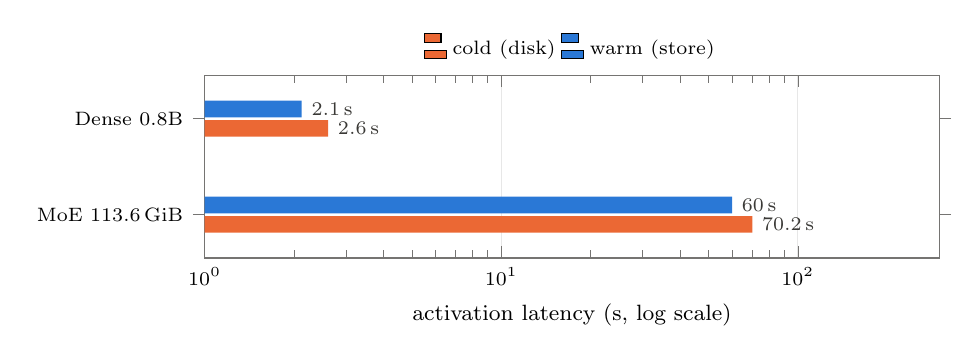
\begin{tikzpicture}
\begin{axis}[paper, width=0.9\columnwidth, height=3.9cm, xbar=1pt, bar width=6pt, xmode=log, log origin=infty,
  xmin=1, xmax=300, xlabel={activation latency (s, log scale)},
  symbolic y coords={MoE,Dense}, ytick={MoE,Dense}, yticklabels={MoE 113.6\,GiB, Dense 0.8B},
  enlarge y limits=0.45, point meta=rawx,
  nodes near coords={\pgfmathprintnumber[fixed,precision=1]{\pgfplotspointmeta}\,s},
  nodes near coords align={horizontal},
  legend style={at={(0.5,1.03)}, anchor=south}, legend columns=2]
\addplot[fill=cB, draw=none] coordinates {(2.61,Dense) (70.2,MoE)};
\addplot[fill=cA, draw=none] coordinates {(2.125,Dense) (60.0,MoE)};
\legend{cold (disk), warm (store)}
\end{axis}
\end{tikzpicture}
\caption{Activation latency from disk and from the prepared store. Dense warm: p50 over 118
activations. The MoE warm activation is dominated by re-copying the mapped n-gram table; with
\code{-{}-ngram-placement disk} its weights load in 6.3--7.6\,s.}
\label{fig:activation}
\end{figure}

Fig.~\ref{fig:activation} shows activation latency. For the dense model, a warm activation takes
2.1\,s (p50; p95 2.2\,s), of which only 0.25\,s is weight upload; the remaining $\sim$1.9\,s are
planning, all-reduce initialization, arena and kernel set-up. For the MoE model the store saves only
10\,s of 70\,s, because the store holds the 67.5\GiB\ of weights ($\approx$6\,s to upload) but the
47.7\GiB\ n-gram table is backed by page cache and is copied again at each activation; since the
store displaces the page cache, that copy comes from disk. Placing the table on disk reduces the warm
weight load to 6.3--7.6\,s. Deactivation takes 0.7\,s (dense) to 1.4\,s (MoE). Switching between two
models that are both already active costs no activation at all.

\subsection{Time to first token}

\begin{table}[t]
\caption{TTFT decomposition, dense 0.8B, 1{,}700-token prompt, p50\,/\,p95 in ms. The parts sum to TTFT within 0.6\,ms.}
\label{tab:ttft}
\centering\footnotesize
\setlength{\tabcolsep}{3.2pt}
\begin{tabular}{@{}lrrrr@{}}
\toprule
Case & Queue & Activation & Prefill & TTFT \\
\midrule
model active        & 0.1\,/\,0.2   & 0              & 23.7\,/\,25.0  & 24.0\,/\,25.5 \\
cold                & 0.5\,/\,0.8   & 1968\,/\,2007  & 37.9\,/\,38.1  & 2008\,/\,2045 \\
prepared (warm)     & 0.4\,/\,0.8   & 2125\,/\,2227  & 28.8\,/\,29.5  & 2155\,/\,2256 \\
32 clients, 8 seqs  & 1403\,/\,1461 & 0              & 27.1\,/\,103.6 & 1431\,/\,1490 \\
\bottomrule
\end{tabular}
\end{table}

Every response reports TTFT split into router wait for activation, scheduler queue and prefill, and
\code{/metrics} exports the same parts as per-model histograms. Table~\ref{tab:ttft} shows that for a
model that is not active, activation is almost the whole TTFT, while for an overloaded active model
the scheduler queue dominates. Activating a second model under that load took as long as without it,
and its own queue stayed below 1\,ms.

\subsection{Concurrent models}

\begin{figure}[t]
\centering
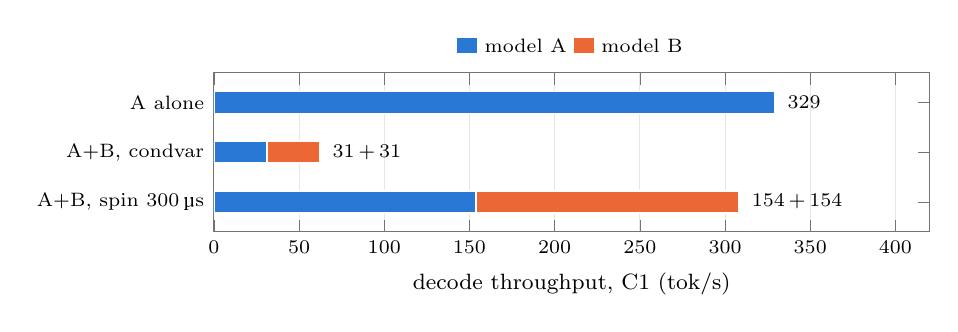
\begin{tikzpicture}
\begin{axis}[paper, width=0.88\columnwidth, height=3.6cm, xbar stacked, bar width=8pt, xmin=0, xmax=420,
  xlabel={decode throughput, C1 (tok/s)},
  symbolic y coords={today,cv,alone}, ytick={today,cv,alone},
  yticklabels={{A+B, spin 300\,\textmu s}, {A+B, condvar}, A alone},
  enlarge y limits=0.3,
  legend style={at={(0.5,1.03)}, anchor=south}, legend columns=2]
\addplot[fill=cA, draw=white, line width=0.6pt] coordinates {(329,alone) (31,cv) (154,today)};
\addplot[fill=cB, draw=white, line width=0.6pt] coordinates {(0,alone) (31,cv) (154,today)};
\node[font=\scriptsize, anchor=west] at (axis cs:331,alone) {329};
\node[font=\scriptsize, anchor=west] at (axis cs:64,cv) {31\,+\,31};
\node[font=\scriptsize, anchor=west] at (axis cs:310,today) {154\,+\,154};
\legend{model A, model B}
\end{axis}
\end{tikzpicture}
\caption{Two dense models busy at once. With a condition-variable hand-off between rank threads,
each model fell to 31\,tok/s; spinning for 300\,\textmu s before sleeping restores the serial bound
of about half the single-model rate each.}
\label{fig:concurrency}
\end{figure}

\begin{table}[t]
\caption{Throughput with two active models (tok/s). ``Busy'' means the other model is under load at the same time.}
\label{tab:concurrent}
\centering\footnotesize
\setlength{\tabcolsep}{3.5pt}
\begin{tabular}{@{}llr@{}}
\toprule
Workload & Configuration & Throughput \\
\midrule
Dense C1      & alone                           & 326--332 \\
              & other model active, idle        & 294--300 \\
              & other model busy                & 154 + 154 \\
Dense C8      & alone                           & 2026--2029 \\
              & both busy                       & 1287--1366 + 716--725 \\
Dense prefill & alone                           & 69{,}000--71{,}000 \\
              & beside busy model               & 36{,}000--47{,}000 \\
MoE C1        & alone (manifest, 1 model)       & 74.8--74.9 \\
              & beside busy dense model         & 59.3--59.4 \\
Two MoE, C8   & one busy / both busy            & 102 / 38.4 + 35.3 \\
\bottomrule
\end{tabular}
\end{table}

Fig.~\ref{fig:concurrency} and Table~\ref{tab:concurrent} quantify the cost of collective ordering.
Two busy dense models obtain about half the single-model decode rate each, so aggregate throughput
stays near the single-model level; the gain is availability, not capacity. A second active but idle
model costs about 10\,\% because execution tapes are bypassed while several engines are registered.
With two MoE models, host RAM is saturated (160\GiB\ of 170\GiB\ in use), and part of the drop
stems from page-cache pressure; the two causes were not separated.

\subsection{Moving memory between models}

\begin{figure}[t]
\centering
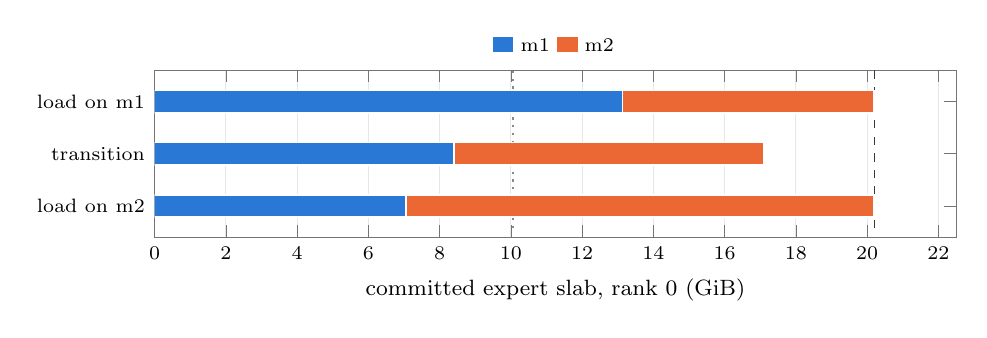
\begin{tikzpicture}
\begin{axis}[paper, height=3.7cm, xbar stacked, bar width=8pt, xmin=0, xmax=22.5,
  xlabel={committed expert slab, rank 0 (GiB)},
  symbolic y coords={p3,p2,p1}, ytick={p3,p2,p1},
  yticklabels={load on m2, transition, load on m1}, enlarge y limits=0.3,
  legend style={at={(0.5,1.02)}, anchor=south}, legend columns=2]
\addplot[fill=cA, draw=white, line width=0.6pt] coordinates {(13.13,p1) (8.41,p2) (7.05,p3)};
\addplot[fill=cB, draw=white, line width=0.6pt] coordinates {(7.06,p1) (8.69,p2) (13.14,p3)};
\draw[ink, dashed] (axis cs:20.20,p3) ++(0pt,-8pt) -- ++(0pt,60pt) node[font=\scriptsize, anchor=south] {pool};
\draw[soft, dotted, thick] (axis cs:10.07,p3) ++(0pt,-8pt) -- ++(0pt,60pt) node[font=\scriptsize, anchor=south, text=soft] {offer};
\legend{m1, m2}
\end{axis}
\end{tikzpicture}
\caption{Elastic expert slab with two Flash-Next entries. The loaded model grows about 3\GiB\ past
its offer while the idle model shrinks to its minimum; the sum never exceeds the pool.}
\label{fig:elastic}
\end{figure}

Fig.~\ref{fig:elastic} shows the elastic slab with two entries of the MoE model, each offering
10.07\GiB\ per rank from a pool of 20.20\GiB. Under load on m1 alone, m1 commits 13.1\GiB\ while m2
falls to 7.1\GiB; reversing the load reverses the split. A change of load reaches its target within
20--30\,s, moving 128\MiB\ per step and 5\GiB\ within a few seconds. Across 7{,}736 samples under a
continuously shifting load, the sum of committed slabs never exceeded the pool (before four fixes,
3{,}561 of 4{,}793 samples did, by up to 3.4\GiB). Greedy outputs of both models matched the
reference after every phase. With KV lending, a cache with a 1.9\GiB\ carve grew by 468--702\MiB\
per card under 12--16 concurrent long prompts while the other model's slab returned 2.8--3.5\GiB, and
it shrank back 13--20\,s after the load, with no lost sequence.

\begin{figure}[t]
\centering
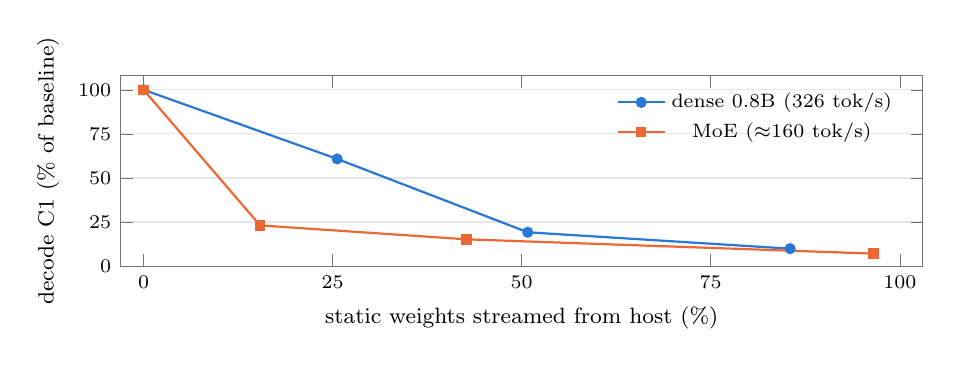
\begin{tikzpicture}
\begin{axis}[paper, height=4.0cm, xmin=-3, xmax=103, ymin=0, ymax=108,
  xlabel={static weights streamed from host (\%)}, ylabel={decode C1 (\% of baseline)},
  ymajorgrids=true, xmajorgrids=false, xtick={0,25,50,75,100}, ytick={0,25,50,75,100},
  legend style={at={(0.98,0.97)}, anchor=north east}]
\addplot[cA, thick, mark=*, mark size=1.6pt] coordinates {(0,100) (25.6,60.8) (50.8,19.2) (85.5,9.9)};
\addplot[cB, thick, mark=square*, mark size=1.5pt] coordinates {(0,100) (15.4,23.1) (42.7,15.2) (96.5,7.1)};
\legend{dense 0.8B (326 tok/s), MoE ($\approx$160 tok/s)}
\end{axis}
\end{tikzpicture}
\caption{Cost of streaming static weights over PCIe, normalized to the non-streaming baseline
(midpoints of min--max ranges). For the MoE model the drop combines streamed statics and experts,
which lose their VRAM slots at the same time.}
\label{fig:streaming}
\end{figure}

Fig.~\ref{fig:streaming} quantifies static-weight streaming. Streaming 25.6\,\% of the dense model's
statics costs 39\,\% of decode throughput, and 85.5\,\% costs 90\,\%; output remains identical, and
throughput recovers within 1--2\,s once VRAM frees up and the weights move back. An activation that
finds the cards full succeeds in every tested case, which is the purpose of streaming: the new model
answers immediately while it waits for memory.

\paragraph{Heat warm-up} For the MoE model, the early expert hit rate (first 64 steps, 246{,}817
routed experts) after a warm re-activation was 83.45\,\% without a warm-up budget and 89.12\,\% with
12\GiB, compared with 83.6\,\% after the cold start.

\subsection{Robustness}

Over 120 activate/deactivate cycles, VRAM returned to 266\MiB\ per card after every cycle; kfd queues,
threads and file descriptors stayed constant, and host RSS grew by at most 17\MiB\ over the last 72
cycles. Failed activations (a model that can never fit, and a malformed container) were rolled back to
the exact pre-activation free VRAM while a 3{,}000-token generation of another model continued
undisturbed. With \code{max\_active\_models}\,=\,2 and three models, each request for the third model
deactivated the longest-idle model and was served after 4.9--5.1\,s. With \code{host\_budget\_mib}
set too low, a second MoE activation was refused with HTTP~503 and no kernel kill.

\subsection{Defects found during acceptance}\label{sec:lessons}

Four defects illustrate where multi-model serving stresses assumptions of a single-model engine.
(i)~\emph{Queue-id exhaustion}: each activation created $\sim$46 AQL streams whose ids were never
reused; the 1{,}024-entry table overflowed at the 23rd activation, surfaced as a misleading
out-of-memory error, and marked the group unhealthy. The table now has $2^{20}$ entries.
(ii)~\emph{Wake-up latency}: the collective hand-off between rank threads used a condition variable
whose sleep--wake cycle cost $\sim$0.5\,ms, 48 times per decode step, reducing two concurrent
models to 31\,tok/s each; spinning for 300\,\textmu s first restored 154\,tok/s.
(iii)~\emph{Mis-counted capacity}: the store's capacity check included the memory-mapped n-gram
table, which is never copied, so the MoE model was never prepared. (iv)~\emph{Virtual-address
aliasing}: on the tested ROCm stack, re-mapping a previously unmapped virtual address had no effect,
so the address kept pointing at its first physical page; once another model owned that page, two
experts aliased and a request occasionally produced no finite logit. Mapping every chunk on fresh
address space removed the error (30 load cycles with external observers, 5{,}776 requests,
0 errors).

% ================================================================ 6 related work
\section{Related Work}\label{sec:related}

\begin{table*}[t]
\caption{RadianceSwap compared with llama-swap, a process-swapping proxy (llama-swap details from its README and example configuration, November 2026).}
\label{tab:llamaswap}
\centering\footnotesize
\renewcommand{\arraystretch}{1.15}
\begin{tabular}{@{}p{3.0cm}p{6.6cm}p{6.6cm}@{}}
\toprule
Aspect & llama-swap~\cite{llamaswap} & RadianceSwap \\
\midrule
Architecture & external reverse proxy (Go) that starts and stops upstream server processes & in-engine, one process (C++/HIP) \\
Backends & any OpenAI- or Anthropic-compatible server (llama.cpp, vLLM, stable-diffusion.cpp, \dots) & Radiance only (\code{.rad} or Hugging Face checkpoint) \\
Platforms & whatever the backend supports; binaries for Linux, macOS, Windows, FreeBSD & Linux, ROCm; evaluated on AMD gfx1201 only \\
Switch & stop process (graceful \code{unloadTimeout}, then kill), start another & tear down runtime; re-activate from the prepared store \\
Warm restart & depends on backend; at best weights in the OS page cache & GPU-ready weights in process memory; no parsing, relayout or disk read \\
Co-residency & one model by default; \code{groups}, a \code{matrix} DSL with eviction costs, or operator-declared \code{capacity} pools & all models by default, bounded by memory budgets \\
VRAM split & fixed per process, declared by the operator & dynamic: group planner, elastic slab, KV lending, static streaming \\
Model does not fit & evict another model & start and stream from host RAM; deactivate idle models \\
Running generations & graceful unload with timeout (not examined here) & never interrupted \\
Multi-GPU & delegated to the backend & one TP group shared by all models, ordered collectives \\
Host memory & not managed & budget, LRU and admission control \\
Maturity & widely deployed, web UI, aliases, request filters, profiles & experimental, one test system \\
\bottomrule
\end{tabular}
\end{table*}

\paragraph{Process-level model swapping} llama-swap~\cite{llamaswap} places a proxy in front of
independent inference servers such as llama.cpp~\cite{llamacpp} and replaces the running server
when a request names another model; operators declare which models may be co-resident. Ollama
similarly loads models on demand and unloads them after a keep-alive period~\cite{ollama}. These
systems are backend-agnostic and portable, which RadianceSwap is not. RadianceSwap's ADR~0001
considered exactly this design, an external router restarting one process per model with weights
warm in the page cache, and rejected it for switch latency and the extra component.
Table~\ref{tab:llamaswap} contrasts the two approaches. A combination is plausible but untested:
since Radiance serves the OpenAI API, a RadianceSwap process could be one upstream of llama-swap.
No benchmark compares the two on the same hardware; the latency advantage of warm in-process
activation follows from the design but was not measured against llama-swap.

\paragraph{Multi-model serving systems} Clockwork~\cite{clockwork} and PipeSwitch~\cite{pipeswitch}
reduce the cost of swapping DNN models on GPUs through predictable scheduling and pipelined
transfer of layers. AlpaServe~\cite{alpaserve} shows that model parallelism enables statistical
multiplexing of several models across devices, and MuxServe~\cite{muxserve} multiplexes several
LLMs spatially and temporally on shared GPUs. ServerlessLLM~\cite{serverlessllm} accelerates
cold starts with a loading-optimized checkpoint format and multi-tier storage. RadianceSwap shares
the goals of fast activation and co-location but operates inside a single engine on a fixed
tensor-parallel group, and adds run-time movement of expert, KV and static-weight memory between
co-located models.

\paragraph{Offloading and memory management} FlexGen~\cite{flexgen} and
DeepSpeed-Inference~\cite{dsinference} offload weights and KV cache to host memory to run models
larger than GPU memory, and Eliseev and Mazur~\cite{eliseev2023} cache MoE experts on the GPU while
offloading the rest. PagedAttention~\cite{vllm} manages the KV cache in blocks to reduce
fragmentation. RadianceSwap reuses Radiance's existing expert tiering and block-paged KV cache and
extends them across model boundaries. S-LoRA~\cite{slora} serves many adapters of one base model;
RadianceSwap instead serves distinct base models and refuses adapters in manifest mode.

% ================================================================ 7 limitations
\section{Limitations and Future Work}

The evaluation covers one system, one MoE model and small dense models; more than two models and
MoE/MoE combinations under an explicit host budget were not tested. All models in a manifest share
one TP size, so plugins that run only with TP\,=\,1 cannot join a TP\,=\,2 group, and the
\code{devices} key is validated but not yet used to select cards. A cold model still reserves its VRAM
share, which can make a large MoE $\sim$9\,\% slower even if the second model never activates
(issue~\#56). A second active model costs $\sim$10\,\% even when idle. KV, prefix and recurrent state
are discarded on deactivation; preserving them in host memory is future work. A long-run check of
the elastic slab after the address-aliasing fix is still open (issue~\#58), as is lending one model's
idle KV blocks to another model's expert slab.

% ================================================================ 8 conclusion
\section{Conclusion}

RadianceSwap shows that multi-model serving can be moved from a process-swapping proxy into the
inference engine itself. Keeping deactivated models GPU-ready in host memory makes re-activation an
upload; ordering collectives makes truly parallel runtimes safe on a tensor-parallel group; and a
heat-driven planner with an elastic slab, KV lending and static streaming lets VRAM follow the load.
On the tested system this costs nothing for a single model, preserves bit-identical outputs, and
turns the wait for a second model from an unbounded drain into seconds. The price is coupling to one
engine and a narrow evaluation, which we hope testers on other hardware will broaden.

% ================================================================ appendix
\appendices
\section{Example manifest}
\begin{lstlisting}
{
 "gpu_group": { "devices": [0, 1], "tp": 2 },
 "cache": {
   "idle_timeout_ms": 300000,
   "warmup_budget_mib": 12288
 },
 "models": [
   { "id": "big", "default": true,
     "path": "/models/big-moe.rad",
     "engine": ["--placement", "expert_tiered",
                "--max-model-len", "16384"] },
   { "id": "small",
     "path": "/models/small",
     "engine": ["--max-model-len", "16384"] }
 ]
}
\end{lstlisting}
Started with \code{radiance -{}-manifest models.json -{}-port 8000}; a request selects a model through
its \code{model} field, and \code{/radiance/models} reports each model's state, VRAM and host
memory. The full reference is \code{docs/GUIDE.md} \S4.12.

% ================================================================ references
\begin{thebibliography}{99}\footnotesize

\bibitem{radiance} Deadcode and the radiance contributors, ``radiance,'' source repository, 2026. [Online]. Available: \url{https://codeberg.org/StillDeadcode/radiance}

\bibitem{llamaswap} mostlygeek, ``llama-swap,'' source repository, 2026. [Online]. Available: \url{https://github.com/mostlygeek/llama-swap}

\bibitem{llamacpp} G.~Gerganov \emph{et al.}, ``llama.cpp,'' source repository. [Online]. Available: \url{https://github.com/ggml-org/llama.cpp}

\bibitem{ollama} Ollama, source repository. [Online]. Available: \url{https://github.com/ollama/ollama}

\bibitem{megatron} M.~Shoeybi, M.~Patwary, R.~Puri, P.~LeGresley, J.~Casper, and B.~Catanzaro, ``Megatron-LM: Training multi-billion parameter language models using model parallelism,'' arXiv:1909.08053, 2019.

\bibitem{shazeer2017} N.~Shazeer, A.~Mirhoseini, K.~Maziarz, A.~Davis, Q.~Le, G.~Hinton, and J.~Dean, ``Outrageously large neural networks: The sparsely-gated mixture-of-experts layer,'' in \emph{Proc. ICLR}, 2017.

\bibitem{fedus2022} W.~Fedus, B.~Zoph, and N.~Shazeer, ``Switch Transformers: Scaling to trillion parameter models with simple and efficient sparsity,'' \emph{J. Mach. Learn. Res.}, vol.~23, no.~120, 2022.

\bibitem{eliseev2023} A.~Eliseev and D.~Mazur, ``Fast inference of mixture-of-experts language models with offloading,'' arXiv:2312.17238, 2023.

\bibitem{flexgen} Y.~Sheng, L.~Zheng, B.~Yuan, Z.~Li, M.~Ryabinin, B.~Chen, P.~Liang, C.~R\'e, I.~Stoica, and C.~Zhang, ``FlexGen: High-throughput generative inference of large language models with a single GPU,'' in \emph{Proc. ICML}, 2023.

\bibitem{dsinference} R.~Y.~Aminabadi, S.~Rajbhandari, A.~A.~Awan, C.~Li, D.~Li, E.~Zheng, O.~Ruwase, S.~Smith, M.~Zhang, J.~Rasley, and Y.~He, ``DeepSpeed-Inference: Enabling efficient inference of transformer models at unprecedented scale,'' in \emph{Proc. SC}, 2022.

\bibitem{havender1968} J.~W.~Havender, ``Avoiding deadlock in multitasking systems,'' \emph{IBM Systems Journal}, vol.~7, no.~2, pp.~74--84, 1968.

\bibitem{denning1968} P.~J.~Denning, ``The working set model for program behavior,'' \emph{Commun. ACM}, vol.~11, no.~5, pp.~323--333, 1968.

\bibitem{clockwork} A.~Gujarati, R.~Karimi, S.~Alzayat, W.~Hao, A.~Kaufmann, Y.~Vigfusson, and J.~Mace, ``Serving DNNs like Clockwork: Performance predictability from the bottom up,'' in \emph{Proc. OSDI}, 2020.

\bibitem{pipeswitch} Z.~Bai, Z.~Zhang, Y.~Zhu, and X.~Jin, ``PipeSwitch: Fast pipelined context switching for deep learning applications,'' in \emph{Proc. OSDI}, 2020.

\bibitem{alpaserve} Z.~Li, L.~Zheng, Y.~Zhong, V.~Liu, Y.~Sheng, X.~Jin, Y.~Huang, Z.~Chen, H.~Zhang, J.~E.~Gonzalez, and I.~Stoica, ``AlpaServe: Statistical multiplexing with model parallelism for deep learning serving,'' in \emph{Proc. OSDI}, 2023.

\bibitem{muxserve} J.~Duan, R.~Lu, H.~Duanmu, X.~Li, X.~Zhang, D.~Lin, I.~Stoica, and H.~Zhang, ``MuxServe: Flexible spatial-temporal multiplexing for multiple LLM serving,'' in \emph{Proc. ICML}, 2024.

\bibitem{serverlessllm} Y.~Fu, L.~Xue, Y.~Huang, A.-O.~Brabete, D.~Ustiugov, Y.~Patel, and L.~Mai, ``ServerlessLLM: Low-latency serverless inference for large language models,'' in \emph{Proc. OSDI}, 2024.

\bibitem{vllm} W.~Kwon, Z.~Li, S.~Zhuang, Y.~Sheng, L.~Zheng, C.~H.~Yu, J.~E.~Gonzalez, H.~Zhang, and I.~Stoica, ``Efficient memory management for large language model serving with PagedAttention,'' in \emph{Proc. SOSP}, 2023.

\bibitem{slora} Y.~Sheng, S.~Cao, D.~Li, C.~Hooper, N.~Lee, S.~Yang, C.~Chou, B.~Zhu, L.~Zheng, K.~Keutzer, J.~E.~Gonzalez, and I.~Stoica, ``S-LoRA: Serving thousands of concurrent LoRA adapters,'' in \emph{Proc. MLSys}, 2024.

\end{thebibliography}

\end{document}
